%%%%%%%%%%%%%%%%%%%%%%%%%%%%%%%%%%%%%%%%%%%%%%%%%%%%%%%%%%%%%%%%%%
%%%%%%%% ICML 2013 EXAMPLE LATEX SUBMISSION FILE %%%%%%%%%%%%%%%%%
%%%%%%%%%%%%%%%%%%%%%%%%%%%%%%%%%%%%%%%%%%%%%%%%%%%%%%%%%%%%%%%%%%

% Use the following line _only_ if you're still using LaTeX 2.09.
%\documentstyle[icml2013,epsf,natbib]{article}
% If you rely on Latex2e packages, like most moden people use this:
\documentclass{article}

% For figures
\usepackage{graphicx} % more modern
%\usepackage{epsfig} % less modern
% \usepackage{subfigure}
\usepackage{subcaption}
\usepackage{multicol}

% For citations
\usepackage{natbib}

% For algorithms
\usepackage{algorithm}
\usepackage{algorithmic}

% For math
\usepackage{amsmath}
\usepackage{siunitx}

% As of 2011, we use the hyperref package to produce hyperlinks in the
% resulting PDF.  If this breaks your system, please commend out the
% following usepackage line and replace \usepackage{icml2013} with
% \usepackage[nohyperref]{icml2013} above.
\usepackage{hyperref}

% Packages hyperref and algorithmic misbehave sometimes.  We can fix
% this with the following command.
\newcommand{\theHalgorithm}{\arabic{algorithm}}

% Employ the following version of the ``usepackage'' statement for
% submitting the draft version of the paper for review.  This will set
% the note in the first column to ``Under review.  Do not distribute.''
\usepackage{icml2013}
% Employ this version of the ``usepackage'' statement after the paper has
% been accepted, when creating the final version.  This will set the
% note in the first column to ``Proceedings of the...''
% \usepackage[accepted]{icml2013}


% The \icmltitle you define below is probably too long as a header.
% Therefore, a short form for the running title is supplied here:
\icmltitlerunning{6.867: Homework 1}

\begin{document}

\twocolumn[
  \icmltitle{6.867: Homework 1}

  % % It is OKAY to include author information, even for blind
  % % submissions: the style file will automatically remove it for you
  % % unless you've provided the [accepted] option to the icml2013
  % % package.
  % \icmlauthor{Your Name}{email@yourdomain.edu}
  % \icmladdress{Your Fantastic Institute,
  %             314159 Pi St., Palo Alto, CA 94306 USA}
  % \icmlauthor{Your CoAuthor's Name}{email@coauthordomain.edu}
  % \icmladdress{Their Fantastic Institute,
  %             27182 Exp St., Toronto, ON M6H 2T1 CANADA}

  % You may provide any keywords that you
  % find helpful for describing your paper; these are used to populate
  % the "keywords" metadata in the PDF but will not be shown in the document
  \icmlkeywords{boring formatting information, machine learning, ICML}

  \vskip 0.3in
]

\section{Gradient descent}

In this section, we explored the simplest and most-commonly discussed method of optimization for differentiable cost functions: gradient descent. We implemented a basic batch gradient descent procedure and applied it to minimize two different objective functions: the negative Gaussian function and the quadratic bowl function. Furthermore, after creating the implementations, we investigated how our choice of starting guess, step size, and convergence criterion/threshold impacted our resulting solution.

\subsection{Starting guess}
In general, we saw that starting guess did not have much of an impact on our resulting solution. If the starting guess was farther away from the actual minimum, it simply took the algorithm more iterations to converge. In the end however, the algorithm would converge for both of our objective functions. It is worth noting however that for alternative objective functions with behavior including plateaus or local minima, starting guess would likely play a larger role. Figure 1 illustrates gradient descent on our two objective functions with starting guesses of various orders of magnitude.

\subsection{Step size}
Throughout our research, we discovered that step size had a fairly significant impact on the resulting solutions. For example, a step size that was too large could result in the gradient descent algorithm diverging instead of converging. This is illustrated in Figure 2 on the right. As we can see, the algorithm oversteps the minimum on the first step which causes the norm of the new gradient to be larger than the original gradient norm. This then proceeded to compound at every step, ultimately causing the algorithm to diverge to infinity.

\subsection{Convergence criterion/threshold}
In addition to step size, the convergence criterion had a fairly significant impact on the resulting solution. In general, we found that accuracy was inversely proportional to the convergence criterion while speed was directly proportional to the convergence criterion, which makes intuitive sense. With a large convergence criterion, the accuracy of the resulting solution was reduced while the algorithm ran to completion faster. On the other hand, with a smaller convergence criterion, the accuracy of the resulting solution was increased while the algorithm took many more iterations to complete. \\ \\

In order to verify that our gradient functions were correct, we created a numerical gradient function so that we could validate the gradients at various points. To calculate the numerical gradients, we utilized the central difference approximation. For the quadratic bowl, it appears that no matter what the difference step was, the numerical gradient was always identical to the true gradient. For the negative gaussian, we discovered that by making the difference step smaller, our numerical gradient gained accuracy and became closer to the true gradient. For example, at the point (0,0), the real gradient for the negative Gaussian was $$[ \num{-1.44009348e-06}, \num{-1.44009348e-06}].$$
The numerical gradient with a difference step of 100 was $$[ \num{-1.14032986e-08} , \num{-1.14032986e-08}].$$
With a difference step of 10, the numerical gradient was $$[ \num{-1.37214353e-06},  \num{-1.37214353e-06}].$$
With a difference step of 1, the numerical gradient was $$[ \num{-1.43939760e-06},  \num{-1.43939760e-06}].$$
Lastly, with a difference step of 0.1, the numerical gradient was
$$[ \num{-1.44008652e-06}, \num{-1.44008652e-06}],$$ which was almost identical to the true gradient. From a mathematical perspective this makes intuitive sense because the definition of a derivative is basically the numerical gradient as the difference step approaches 0. \\ \\

In the next part of our research, we utilized two forms of gradient descent (batch and stochastic gradient descent) in order to minimize the following function: \\
$$J(\theta) = \Sigma_{i}(x^{(i)T}\theta - y^{i})^2$$

As before, we had to be very particular in the convergence criterion and step sizes in order to ensure that the gradient descent converged. For batch gradient descent, we chose an initial guess of all $0$'s with a step size of $10^{-6}$ and a convergence criterion of 1. This resulted in a $\theta$ that converged to [0.50832359, -2.33986133, -6.31150421, 6.80803415, -1.06442692, 6.66532056, 3.39605963, -0.45908695, -12.94348103, 15.73213395], which ultimately gave a minimum $J(\theta)$ of $8343.21291982$. \\ \\

In stochastic gradient descent, instead of evaluating all training data in every parameter update, each update is based on a single training sample. When specifying the learning rate for each step, we used the Robbins-Monro conditions in order to guarantee convergence. Specifically, in our update rule
$$\theta_{t+1} = \theta_{t} - \eta_{t}\nabla_{\theta}J(\theta_t; x^{(i)}, y^{(i)}),$$
we define
$$\eta_t = (\tau_0 + t)^{-\kappa}$$
where $\kappa = 0.75$ and $\tau_{0} = 10^{8}$. In terms of accuracy, the batch gradient descent was generally more accurate than the stochastic gradient descent. However, in terms of the number of evaluations, the stochastic requires fewer iterations per parameter update. This is because in each iteration of batch gradient descent, $n$ evaluations are necessary, compared with stochastic gradient descent which evaluates the a single point-wise gradient per update iteration. Overall however, we found that batch gradient descent required fewer overall evaluations than stochastic gradient descent.

\section{Linear basis function regression}

We consider linear basis function regression as a method to benchmark the robustness of the gradient descent solution presented above. By using the closed-form maximum likelihood equation, we can calculate the maximum likelihood weight vector for our list of basis functions to approximate the data in the form of our basis. In this scenario, we are using data generated by $y(x) = \cos(\pi x) + 1.5 \cos(2 \pi x) + \epsilon(x)$, where $\epsilon(x)$ is some added noise to the dataset. Running linear regression on a simple polynomial basis of order $M$, where $\phi_0(x) = x^0$, $\phi_1(x) = x^1$, $\phi_2(x) = x^2$, ..., $\phi_M(x) = x^M$, we calculate the maximum likelihood weight vector by the following:
$$w_{ML} = (\Phi^T \Phi)^{-1} \Phi^T y$$
where $w_{ML}$ is the maximum likelihood weight vector and $\Phi$ is given by:
$$\Phi =
\begin{bmatrix}
  \phi_0(x_0)   & \phi_1(x_0)   & \phi_2(x_0)   & \dots   & \phi_M(x_0) \\
  \phi_0(x_1)   & \phi_1(x_1)   & \phi_2(x_1)   & \dots   & \phi_M(x_1) \\
  \vdots        & \vdots        & \vdots        & \ddots  & \vdots \\
  \phi_0(x_n)   & \phi_1(x_n)   & \phi_2(x_n)   & \dots   & \phi_M(x_n) \\
\end{bmatrix}
$$
Our choice of $M$, the degree of our polynomial basis, largely determines the fit of the regression to the data (Figure 2). More specifically, as small values of $M$, the polynomial basis cannot adequately capture all the data points. At higher values of $M$ however, overfitting occurs in which the weight vector performs well on the training data, but is not well generalized to new data. The value of $M$ therefore must be carefully considered in order to prevent too high variability in our generated regression polynomial. \\
\begin{figure}[width=\linewidth]
\centering
\begin{multicols}{2}
  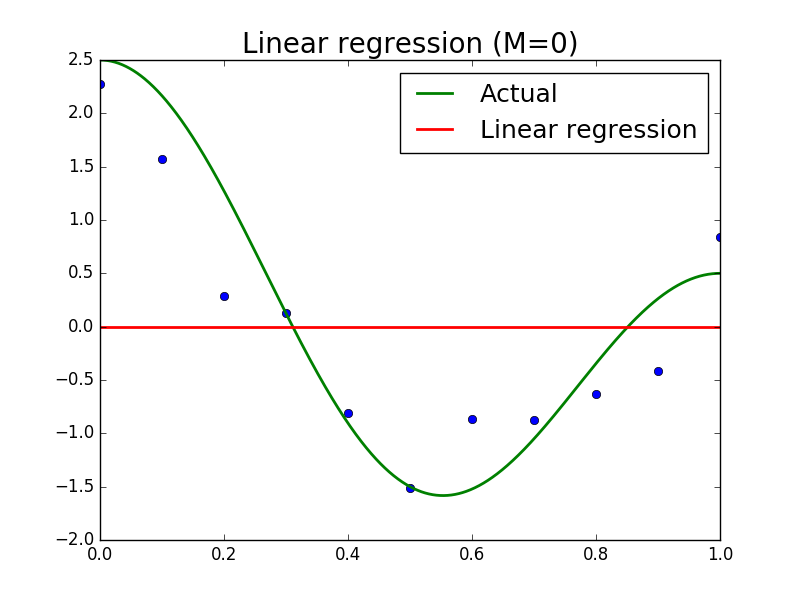
\includegraphics[width=1.2\linewidth]{code/P2/linear_regression,0.png}
  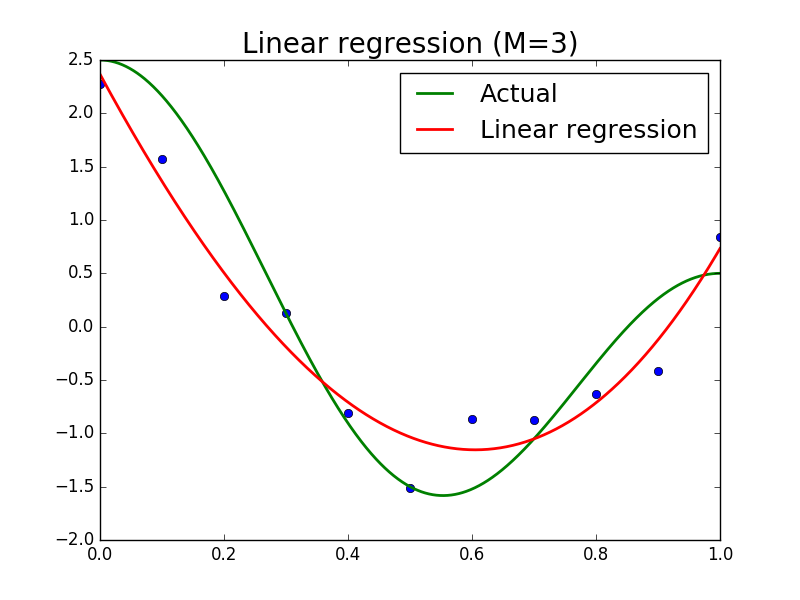
\includegraphics[width=1.2\linewidth]{code/P2/linear_regression,3.png}
  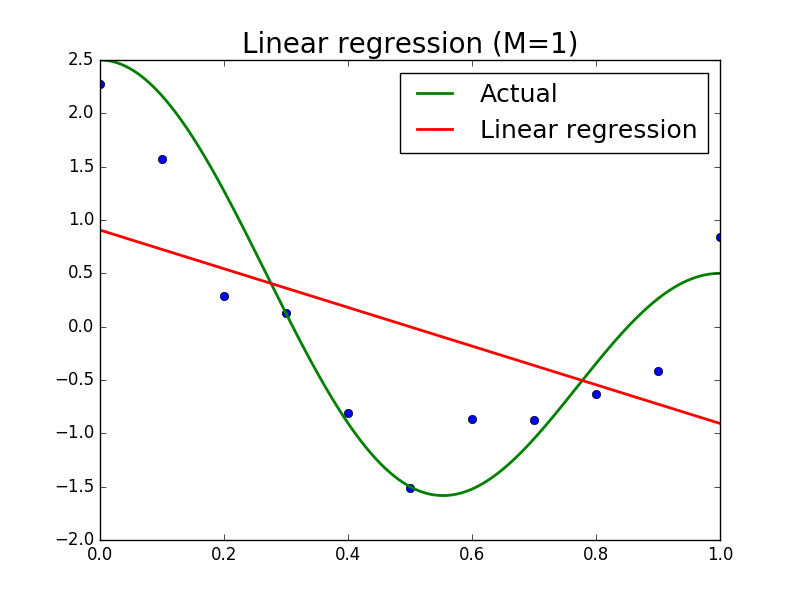
\includegraphics[width=1.2\linewidth]{code/P2/linear_regression,1.png}
  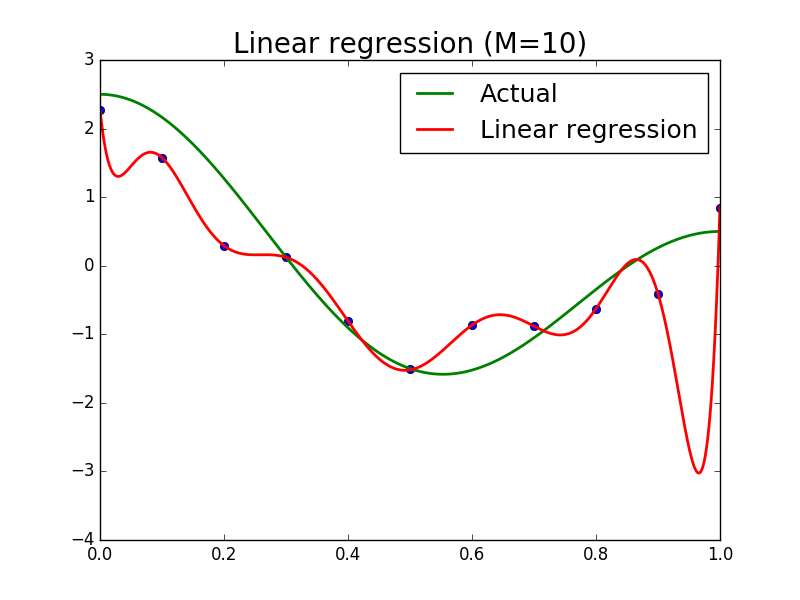
\includegraphics[width=1.2\linewidth]{code/P2/linear_regression,10.png}
\end{multicols}
\caption{Linear regression for varying values of M.}
\end{figure}

After using the closed-form solution to determine the optimum weights for a given $M$, we then proceeded to reproduce these weights through batch and stochastic gradient descent. In order to use gradient descent we needed an objective function which was simply the sum of squares error function. To create the function we would multiply together the $x$ input and the weight vector to get a guess and then find the difference between this guess and the actual $y$ value. We then squared this difference and summed up all these squared differences throughout the entire dataset. To find the gradient we simply took the derivative of this loss function and verified its accuracy with the numeric gradient. We discovered at multiple $M$ values and weight vectors that the gradients were consistent with one another meaning that our calculated gradient was correct. Due to the nature of the fact that the dataset was created by a cosine function we found that choosing $M = 1$ gave a much larger loss than choosing $M = 2/3$ (basically an order of magnitude of difference). We made the following observations regarding the impact of initial guess, step size, and convergence thresholds on batch gradient descent for $M$ values of 2 and 3. \\

Initial guess size:\\
The overall findings we made regarding initial guess size is that as the initial guess size increases exponentially, the number of steps needed to converge only increases linearly. Furthermore, the initial guess size does not have any impact on the actual resulting converged weight (which was  [2.393, -11.767, 9.969]. For example, with $M = 2$, and an initial guess of [100, 100, 100] the algorithm converged in 626 steps. Then with an initial guess of [1000, 1000, 1000] the algorithm converged in 1178 steps. Then with an initial guess of [10000, 10000, 10000], the algorithm converged in 1790 steps. The one minor interesting thing we found is that with an initial guess size of [1, 1, 1]  it actually took 817 steps which is more than [100, 100, 100] even though it's closer to the actual converged weights. Our hypothesis for this strange phenomenon is that since some components of our initial guess were smaller than the converged value and come were greater, this requires more steps than when all components of the initial guess are larger.\\

Step size: \\
We actually made some pretty interesting findings regarding the impact of step size on our gradient descent convergence. Using $M = 2$, the true weights are [2.456, -12.150, 10.338]. We found that a step size equal to or above $0.07$ resulted in a divergent solution. For a step size of $0.06$. we got a converged weight of [2.398, -11.799, 10.001] which is quite close to the actual weights. The convergence graph at this particular step size is shown to the right. As you can see, an interesting phenomenon occurs in that the gradient is descended in an oscillatory manner instead of just the standard one side method. At step sizes smaller than $0.06$, we actually found the converged weight to be less accurate. For example, at a step size of $0.006$ we get a converged weight of [2.255, -10.929, 9.160]. At first this is a bit counterintuitive because one would assume that a smaller step size would result in more fine-tuning and more accuracy. However, if we think about it a bit more we realize that a smaller step size may actual reduce accuracy because the convergence threshold is met faster.\\

\begin{figure}[width=\linewidth]
\centering
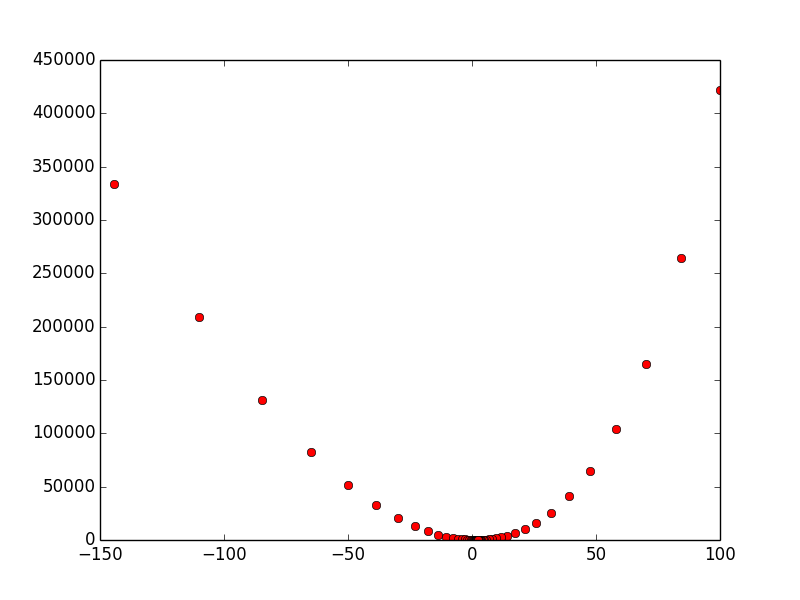
\includegraphics[width=1.2\linewidth]{code/P2/oscillation.png}
\caption{Linear regression for varying values of M.}
\end{figure}

Convergence threshold:\\
The overall findings we made regarding convergence threshold is that larger convergence thresholds meant less steps and less accuracy in the converged weights as compared to the true weights calculated using the closed form solution. Using $M = 2$, the true weights are [2.456, -12.150, 10.338]. At a convergence threshold of 0.0001, the converged weight is [2.393, -11.767, 9.969]. At a convergence threshold of 0.001, the converged weight is [2.657, -13.367, 11.504] (clearly farther away from the true weights). At a convergence threshold of 0.1, the converged weight is [3.978, -20.651, 18.206] (extremely far from the true weights).\\

Batch Gradient Descent vs Stochastic Gradient Descent: \\

When we compared performance of SGD with Batch, we found that for both $M = 1$ and $M = 2$, SGD was able to converge to a more accurate weight in less single-point evaluation steps. For $M = 2$, the true weights are [2.456, -12.150, 10.338]. As mentioned before, it takes Batch gradient descent (with optimum step size of 0.06) 626 steps (6886 single point evaluations) to converge to [2.398, -11.799, 10.001]. On the other hand, SGD (with $k = 6$ and $t_{0} = 100$) is able to converge to [ 2.434, -12.0154  10.208] with only 2679 single point evaluations. A similar phenomenon was noticed with $M = 1$. 

We can also instead choose our set of basis functions to be the set of cosine functions, where $\phi_1(x) = \cos(\pi x)$, $\phi_2(x) = \cos(2 \pi x)$, ..., $\phi_M(x) = \cos(M \pi x)$. This is again calculated for multiple values of $M$ and compared in Figure 3. Interestingly, even when we use the same family of basis functions as used to generate the initial data ($M=2$), due to the noise $\epsilon(x)$ added to the initial dataset, the maximum likelihood weight vector does not identically match the actual function used:
$$ w =
\begin{bmatrix}
  1 \\
  1.5
\end{bmatrix}$$
$$ w_{MLE} =
\begin{bmatrix}
  0.779 \\
  1.174
\end{bmatrix}$$
where $w$ is the actual weight vector and $w_{MLE}$ is the maximum likelihood estimated weight vector.

\begin{figure}[width=\linewidth]
\centering
\begin{multicols}{2}
  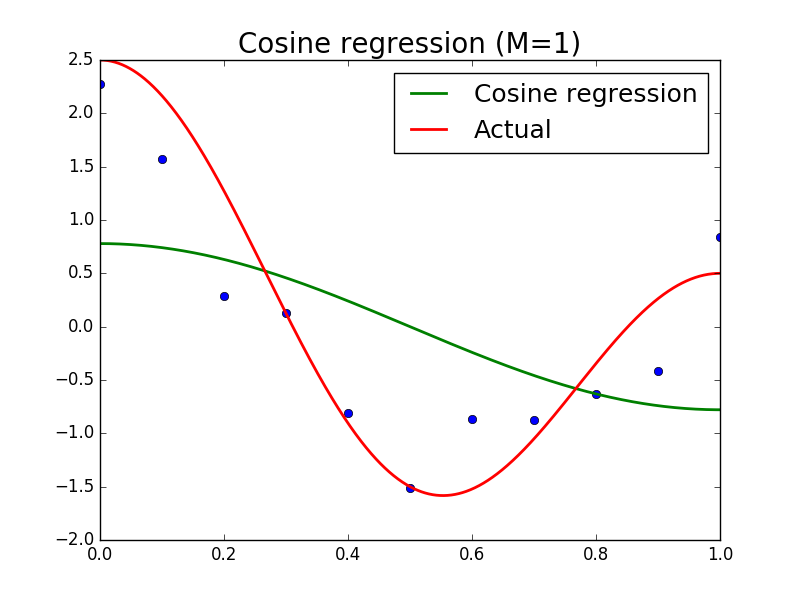
\includegraphics[width=1.2\linewidth]{code/P2/cosine_regression,1.png}
  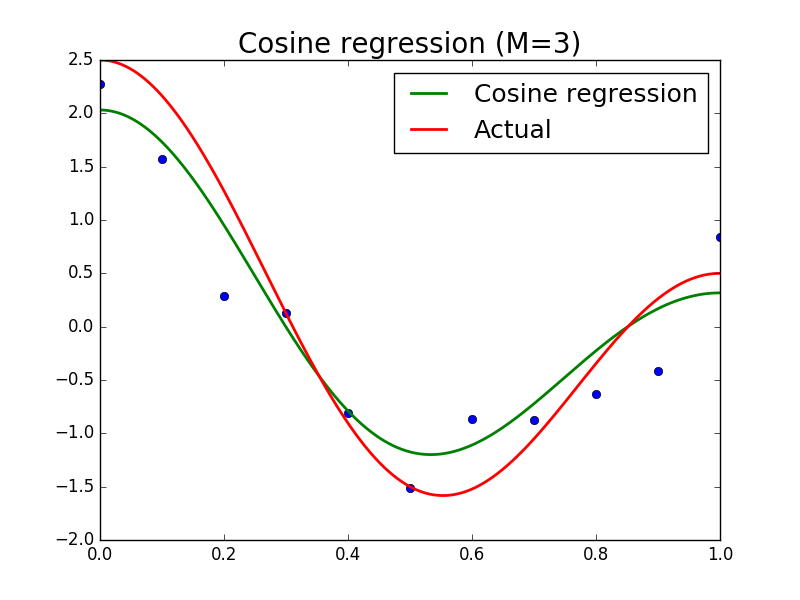
\includegraphics[width=1.2\linewidth]{code/P2/cosine_regression,3.png}
  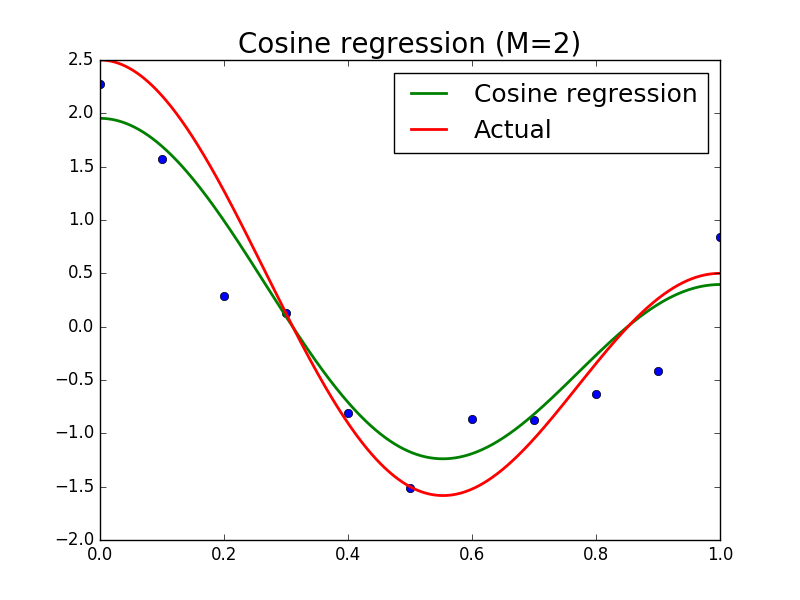
\includegraphics[width=1.2\linewidth]{code/P2/cosine_regression,2.png}
  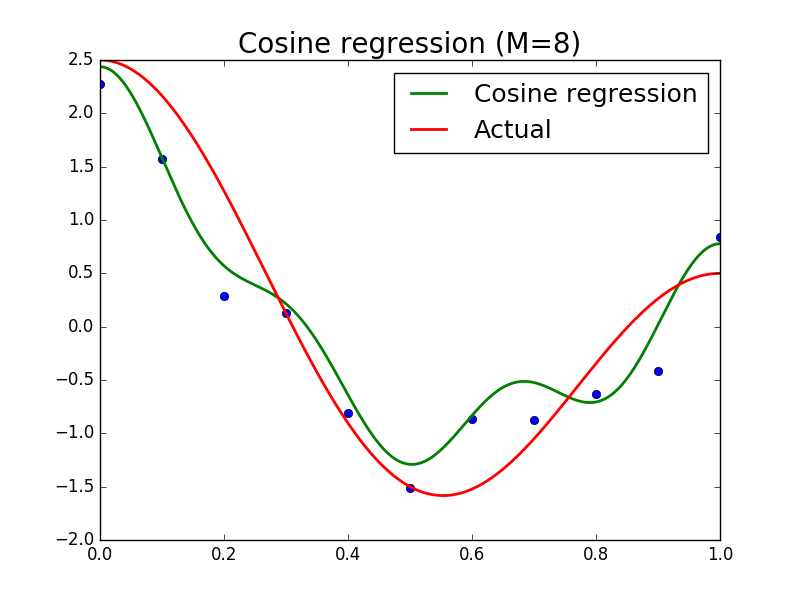
\includegraphics[width=1.2\linewidth]{code/P2/cosine_regression,8.png}
\end{multicols}
\caption{Linear regression for varying values of M.}
\end{figure}
\vspace{3mm}

\section{Ridge regression}

As illustrated in the previous section, some values of $M$ can result in overfitting to the training set. Thus, in an attempt to reduce overfitting, we implement ridge regression, which adds a regularization parameter $\lambda$ to the regression function. In this case, we have chosen a regularizer to serve as a weight decay, in order to encourage weight vector values to tend towards zero unless otherwise supported by the data. For any given value of $M$ therefore, with greater weight decay regularization coefficients, the weight vector decays more strongly towards zero. In other words, for higher values of $\lambda$, the data must more strongly support greater weight vector values in order to acehive the same magnitude of coefficients in the weight vector. \\ \\
This is illustrated in Figure 4, where the first row illustrates the fit of ridge regression using a polynomial basis of degree 3 with $\lambda = 0.1$ and $1$ and the second row shows the fit of the ridge regression using a polynomial basis of degree 10. As illustrated, the weight vector coefficients in the regression are dampened towards zero with greater values of the regularization coefficient. This is compared with the regression computed with a $\lambda = 0$ to illustrate the decay effect of the regulaization parameter. \\ \\

\begin{figure}[width=\linewidth]
\centering
\begin{multicols}{2}
  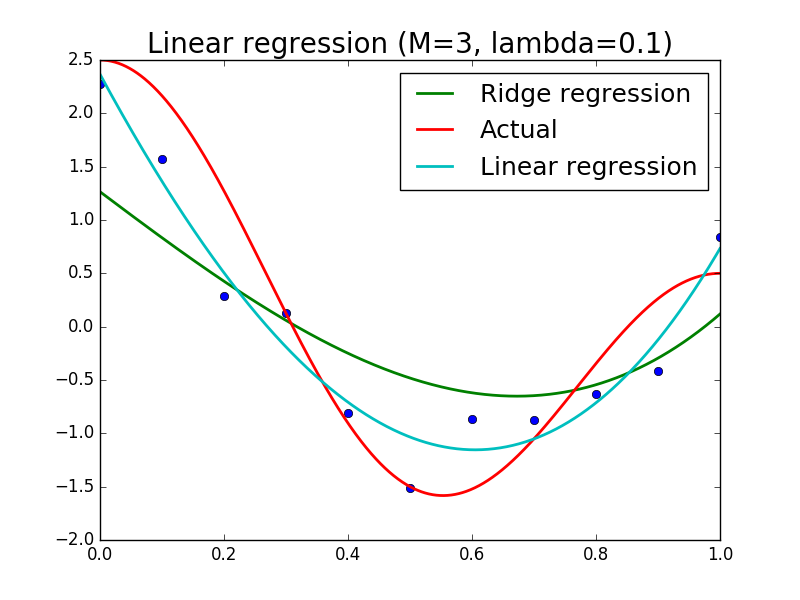
\includegraphics[width=1.2\linewidth]{code/P3/ridge_regression,3,01.png}
  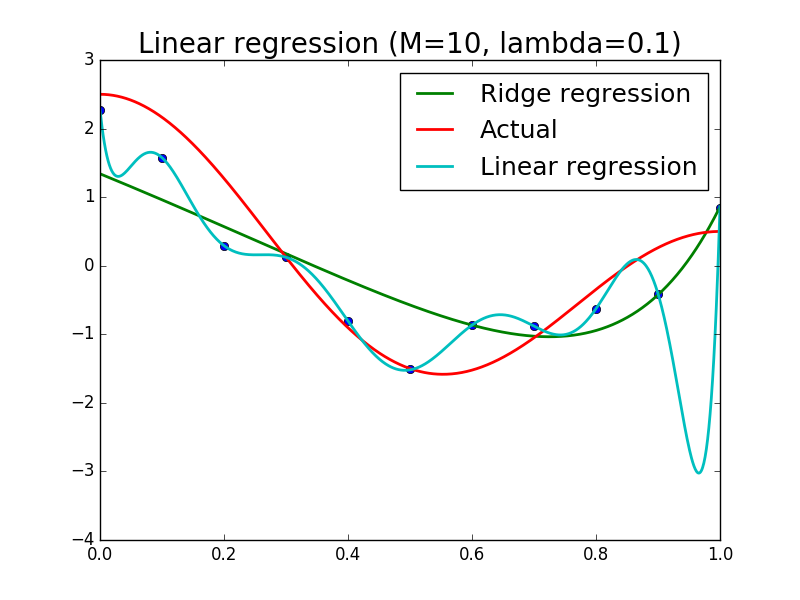
\includegraphics[width=1.2\linewidth]{code/P3/ridge_regression,10,01.png}
  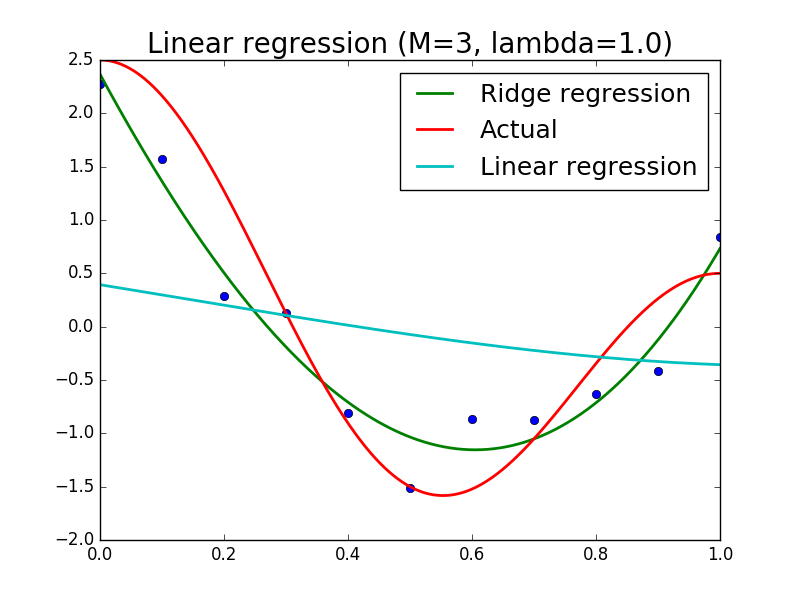
\includegraphics[width=1.2\linewidth]{code/P3/ridge_regression,3,1.png}
  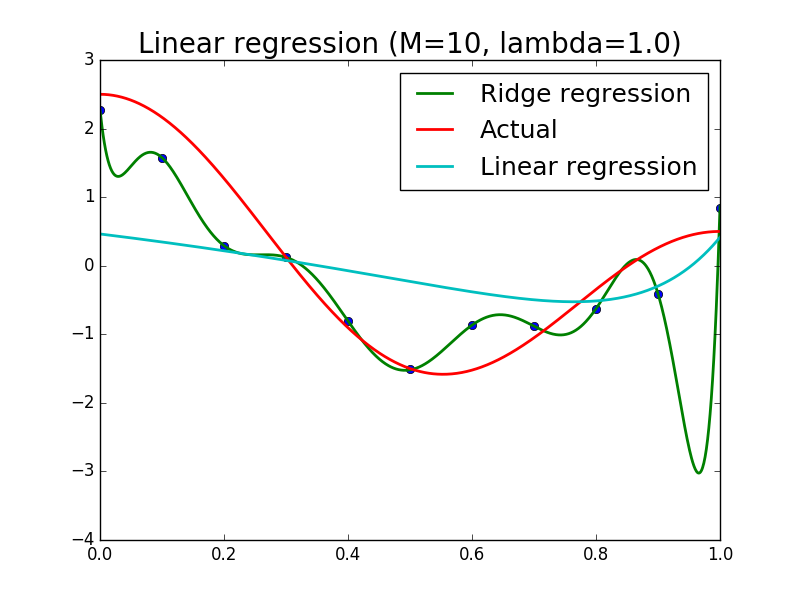
\includegraphics[width=1.2\linewidth]{code/P3/ridge_regression,10,1.png}
\end{multicols}
\caption{Ridge regression for values of M and $\lambda$.}
\end{figure}

Using additional data sets for validation and testing, we can select for the best $M$ and $\lambda$ parameters in our regression model using a polynomial basis. More specifically, for many combinations of values of $M$ and $\lambda$, the maximum likelihood weight vector $w_{MLE}$ was calculated based on the training data set. Through model selection on the validation data set, the best model and optimal values for $M$ and $\lambda$ were chosen based on the evaluation metric. This optimal regression model was then run on the testing data set to evaluate the performance of the model on the new data. The maximum likelihood weight vectors were generated for all $M \in [0, 10]$ and $\lambda \in \{0, 0.1, 0.2, ..., 1.4, 1.5\}$, and this was performed multiple times with data set A as the training data and data set B as the testing data, as well as vice versa. The performance of the regression model was evaluated using the sum of squared errors (SSE) and the mean squared errors (MSE); qualitatively, both evaluation metrics result in the same conclusions, although quantitatively, some additional information can be gleaned from each evaluation metric. \\ \\
When data set A was used as the training data and data set B was used as the testing data, the validation step indicated that $M = 2$ and $\lambda=0.0$ yielded the optimal regression model with a minimum SSE of $2.35$ and a minimum MSE of $0.11$. Running this model on the testing data demonstrated that the regression fit the testing data remarkably well, excepting a single outlier in the testing data. Thus, despite a relatively low MSE of $2.58$ on the testing data, the SSE was relatively high at $25.75$ due to the significant error in the outlier data point. The training, validation, and testing steps are illustrated in Figure 6, in which the best regression line chosen in model selection is plotted against each data set used for training, validation, and testing, respectively. \\ \\

\begin{figure}[width=\linewidth]
\centering
\begin{multicols}{2}
  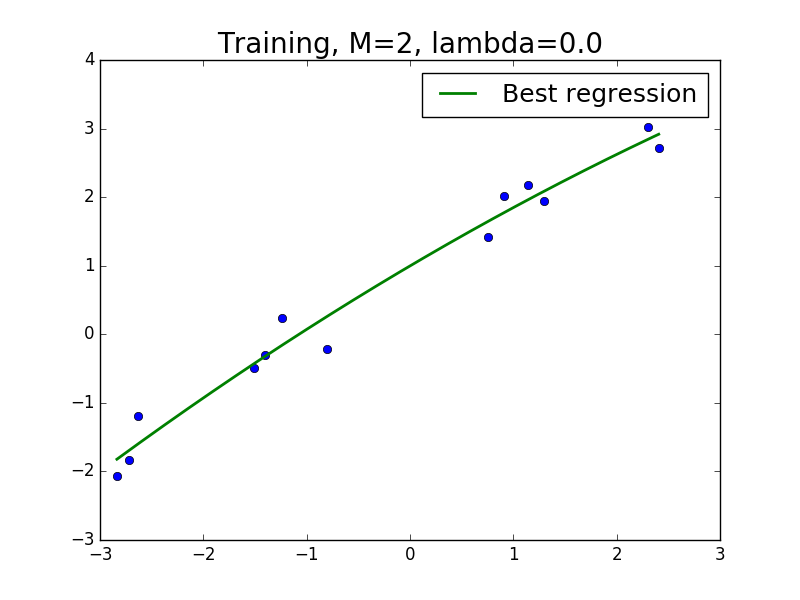
\includegraphics[width=1.2\linewidth]{code/P3/training,training_a,testing_b.png}
  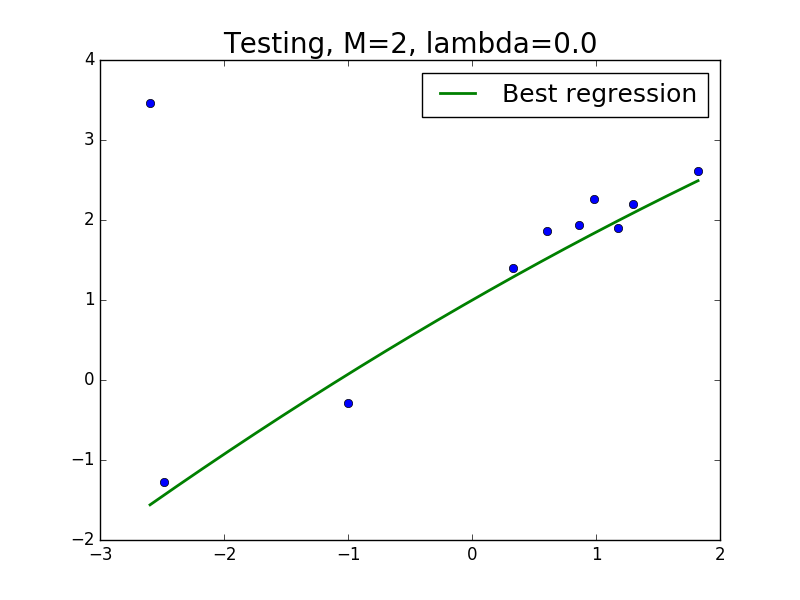
\includegraphics[width=1.2\linewidth]{code/P3/testing,training_a,testing_b.png}
  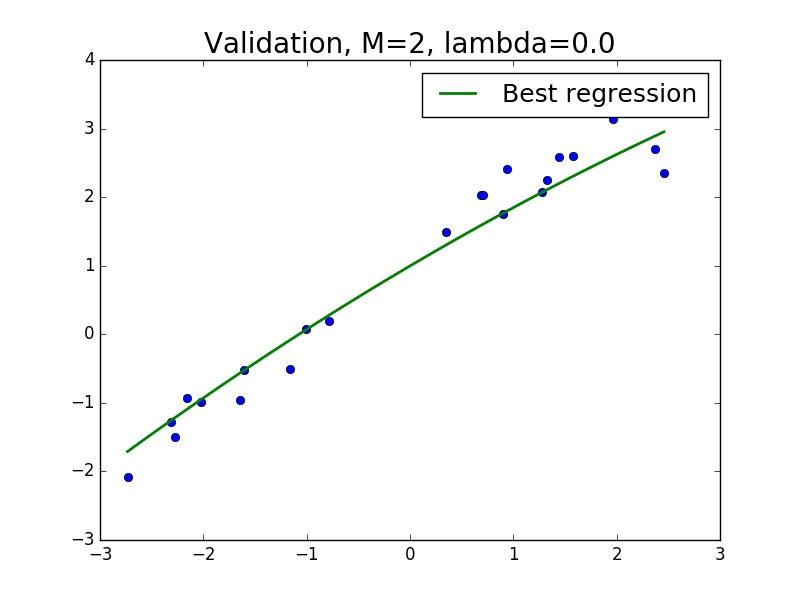
\includegraphics[width=1.2\linewidth]{code/P3/validation,training_a,testing_b.png}
\end{multicols}
\caption{Training on data A, testing on data B.}
\end{figure}

When data set B was used as the training data and data set A was used as the testing data, the validation step indicated that $M = 3$ and $\lambda=0.6$ gave the optimal regression model with a minimum SSE of $28.10$ and minimum MSE of $1.28$. In this case, as the model and maximum likelihood weight vectors were computed based on the data set with the outlier data point, the model was trained to try to account for this outlier data point as well. Thus, during the validation step during model selection, the minimum SSE and MSE were significantly greater than when the data set without the outlier was used for training. This can additionally be seen in the testing step, in which the SSE was $40.09$ and the MSE was $3.08$. This regression model on the training, validation, and testing data sets is again visualized in Figure 7. \\ \\

\begin{figure}[width=\linewidth]
\centering
\begin{multicols}{2}
  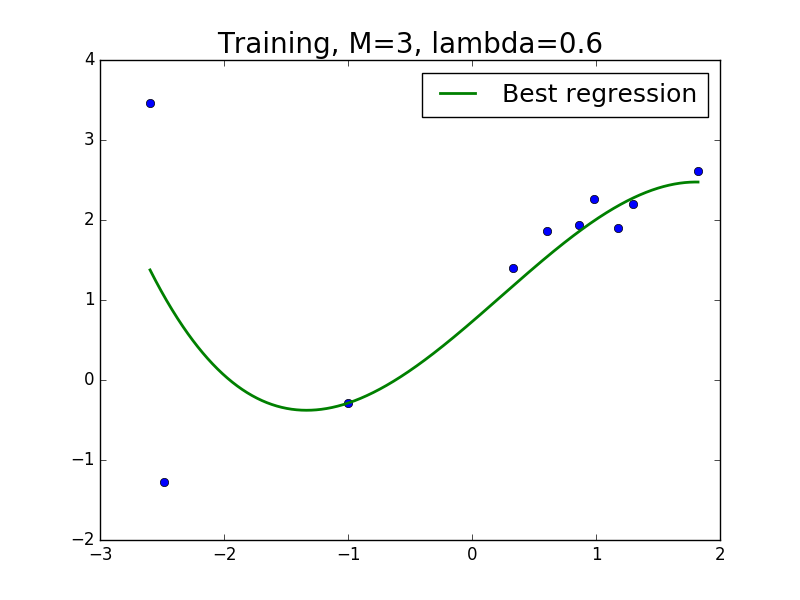
\includegraphics[width=1.2\linewidth]{code/P3/training,training_b,testing_a.png}
  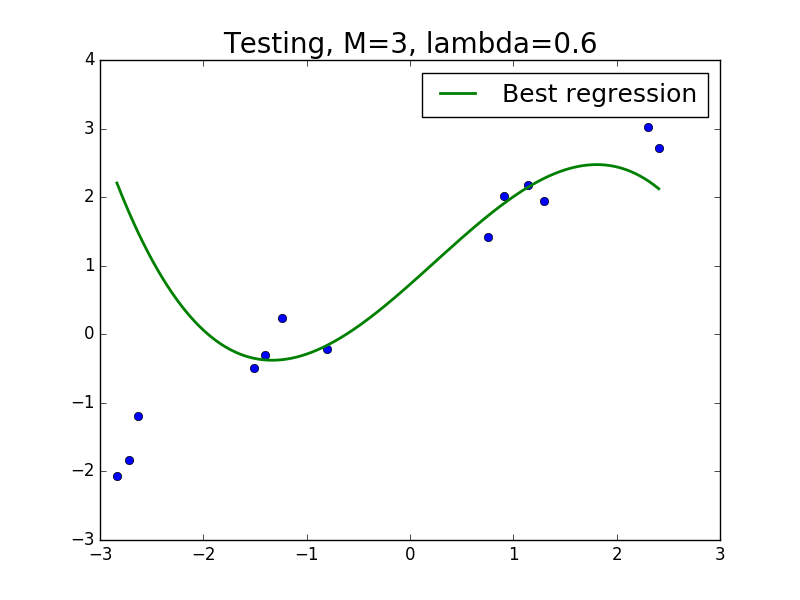
\includegraphics[width=1.2\linewidth]{code/P3/testing,training_b,testing_a.png}
  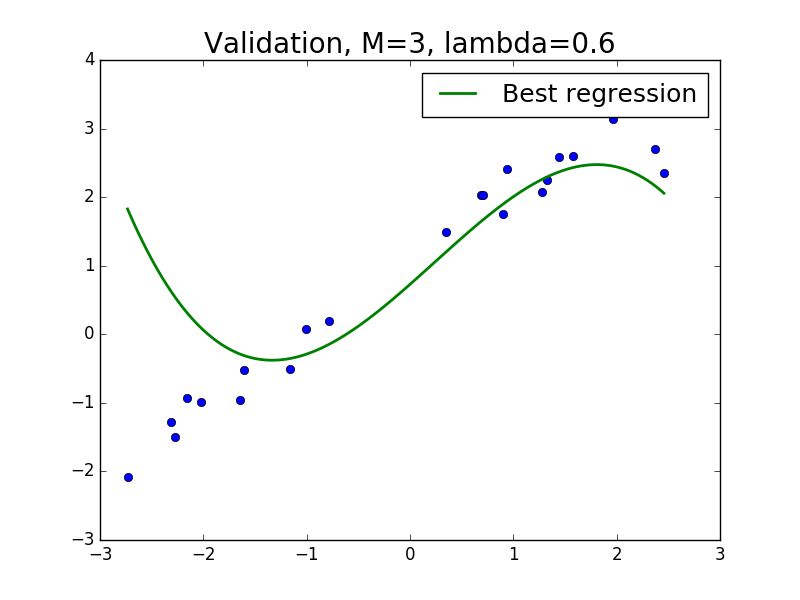
\includegraphics[width=1.2\linewidth]{code/P3/validation,training_b,testing_a.png}
\end{multicols}
\caption{Training on data B, testing on data A.}
\end{figure}

Under both evaluation metrics (SSE and MSE), we can conclude that the polynomial basis yielded better linear regression when trained on data set A and tested on data set B. By examining and comparing both metrics however, we can gain additional information regarding the spread of the data and any potential outliers. This makes intuitive sense when considering the roles of training, validation, and testing and allows us to draw conclusions about the relationships and relative importance of each step with respect to each other.

\section{Sparsity and LASSO}
In this section of our research, we begin to tackle problems where the closed-form solutions do not exist. Specifically, we use the LASSO estimator to try and estimate the true weights for a dataset generated by the following function: \\ 

$$y = w^{T}_{true}\phi(x)+\epsilon$$ (The $\epsilon$ simply represents small noise. Furthermore, the feature vector is give by the following equation:\\

$$\phi(x) = (x,sin(0.4\pi x \times 1), sin(0.4\pi x \times 2), . . . , sin(0.4\pi x \times 12))$$\\

The true parameter $w^{T}_{true}$ was given to us as [0.000000000000000000e+00 0.000000000000000000e+00 5.646300000000000100e+00 7.785999999999999600e-01 0.000000000000000000e+00 8.108999999999999500e-01 2.682700000000000100e+00 0.000000000000000000e+00 0.000000000000000000e+00 0.000000000000000000e+00 0.000000000000000000e+00 0.000000000000000000e+00 0.000000000000000000e+00]. As you can see there are only 4 non-zero components to this vector meaning that it is quite sparse. (Sparseness just means that there are only a few components of the vector that are non-zero and in general sparse weights mean that the algorithm is able to calculate the value of the function faster.  \\

The overarching idea was that we would be able to attain the sparseness using LASSO because the regularization penalty used in LASSO is the $L_{1}$ norm. In terms of actual implementation, we decided to use the Lasso function from sklearn. Ultimately, we were indeed able to get a sparse estimation from LASSO. With the following weights: [ need to fill in ] we were able to get a pretty good estimation of the actual curve that was created from the true weights. You can see how similar the graphs are in the pictures on the right.


\end{document}


% This document was modified from the file originally made available by
% Pat Langley and Andrea Danyluk for ICML-2K. This version was
% created by Lise Getoor and Tobias Scheffer, it was slightly modified
% from the 2010 version by Thorsten Joachims & Johannes Fuernkranz,
% slightly modified from the 2009 version by Kiri Wagstaff and
% Sam Roweis's 2008 version, which is slightly modified from
% Prasad Tadepalli's 2007 version which is a lightly
% changed version of the previous year's version by Andrew Moore,
% which was in turn edited from those of Kristian Kersting and
% Codrina Lauth. Alex Smola contributed to the algorithmic style files.
